\documentclass{labreport}

\begin{document}

\labtitle
    {3}
    {Empirical Analysis of Graph Traversal Algorithms: DFS and BFS}
    {st. gr. FAF-243}
    {Ilie Covali}
    {asist. univ. Fistic Cristofor}

% Table of contents
\tableofcontents
\newpage

\section{ALGORITHM ANALYSIS}

\subsection{Objective}
Study and analyze Breadth First Search (BFS) and Depth First Search (DFS) using empirical measurements.

\subsection{Tasks}
\begin{enumerate}
    \item Implement BFS and DFS in a programming language;
    \item Establish the properties of the input data against which the analysis is performed;
    \item Choose metrics for comparing the algorithms;
    \item Perform empirical analysis of the proposed algorithms;
    \item Make a graphical presentation of the obtained data;
    \item Formulate conclusions based on the performed work.
\end{enumerate}

\subsection{Theoretical Notes}
Breadth First Search and Depth First Search are fundamental graph traversal algorithms. For a graph represented with adjacency lists, both have theoretical time complexity $O(V + E)$, where $V$ is the number of vertices and $E$ is the number of edges.

BFS explores the graph level by level from a start vertex using a queue. This makes it suitable for shortest paths in unweighted graphs.

DFS explores a path as deep as possible before backtracking, usually implemented with recursion or a stack. It is useful in connectivity checks, topological ordering, and cycle detection.

Although both algorithms have the same asymptotic complexity, practical runtime differs because of data structure overheads and memory access patterns.

\subsection{Comparison Metric}
The selected metric is average execution time in seconds for traversing each graph, measured with \texttt{time.perf\_counter()} and averaged over multiple runs.

\subsection{Input Format}
The input for each algorithm is a connected, undirected sparse graph represented implicitly.

Input properties used in the experiments:
\begin{itemize}
    \item Number of vertices sampled from 1000 up to 1000000 (24 input sizes);
    \item Each vertex $i$ has neighbors $(i \pm 1)$, $(i \pm 2)$, $(i \pm 3)$ modulo $n$;
    \item The resulting graph is connected and has constant degree 6;
    \item 5 timed traversals per input size (average reported).
\end{itemize}

\newpage
\section{IMPLEMENTATION}

Both algorithms were implemented in Python. To avoid recursion depth limitations for large graphs, DFS was implemented iteratively with an explicit stack. For scalability up to one million vertices, neighbors are computed on demand instead of storing full adjacency lists.

\subsection{Breadth First Search (BFS)}

\subsubsection{Algorithm Description}
The algorithm starts from a source node, marks it as visited, then repeatedly extracts a node from a queue and visits all of its unvisited neighbors.

Pseudocode:
\begin{verbatim}
BFS(graph, start):
    visited[start] <- true
    queue <- [start]
    while queue is not empty:
        u <- pop_front(queue)
        for each v in graph[u]:
            if not visited[v]:
                visited[v] <- true
                push_back(queue, v)
\end{verbatim}

\subsubsection{Implementation}
\begin{lstlisting}[style=python, caption={BFS implementation in Python}]
from collections import deque

DEGREE_STEPS = (1, 2, 3)

def bfs(node_count, start=0):
    node_count = int(node_count)
    if node_count <= 0:
        return 0

    start = int(start) % node_count
    visited = bytearray(node_count)
    queue = deque([start])
    visited[start] = 1
    visited_count = 0

    while queue:
        node = queue.popleft()
        visited_count += 1
        for step in DEGREE_STEPS:
            n_plus = (node + step) % node_count
            n_minus = (node - step) % node_count
            if not visited[n_plus]:
                visited[n_plus] = 1
                queue.append(n_plus)
            if not visited[n_minus]:
                visited[n_minus] = 1
                queue.append(n_minus)

    return visited_count
\end{lstlisting}

\subsubsection{Results}
\begin{figure}[H]
    \centering
    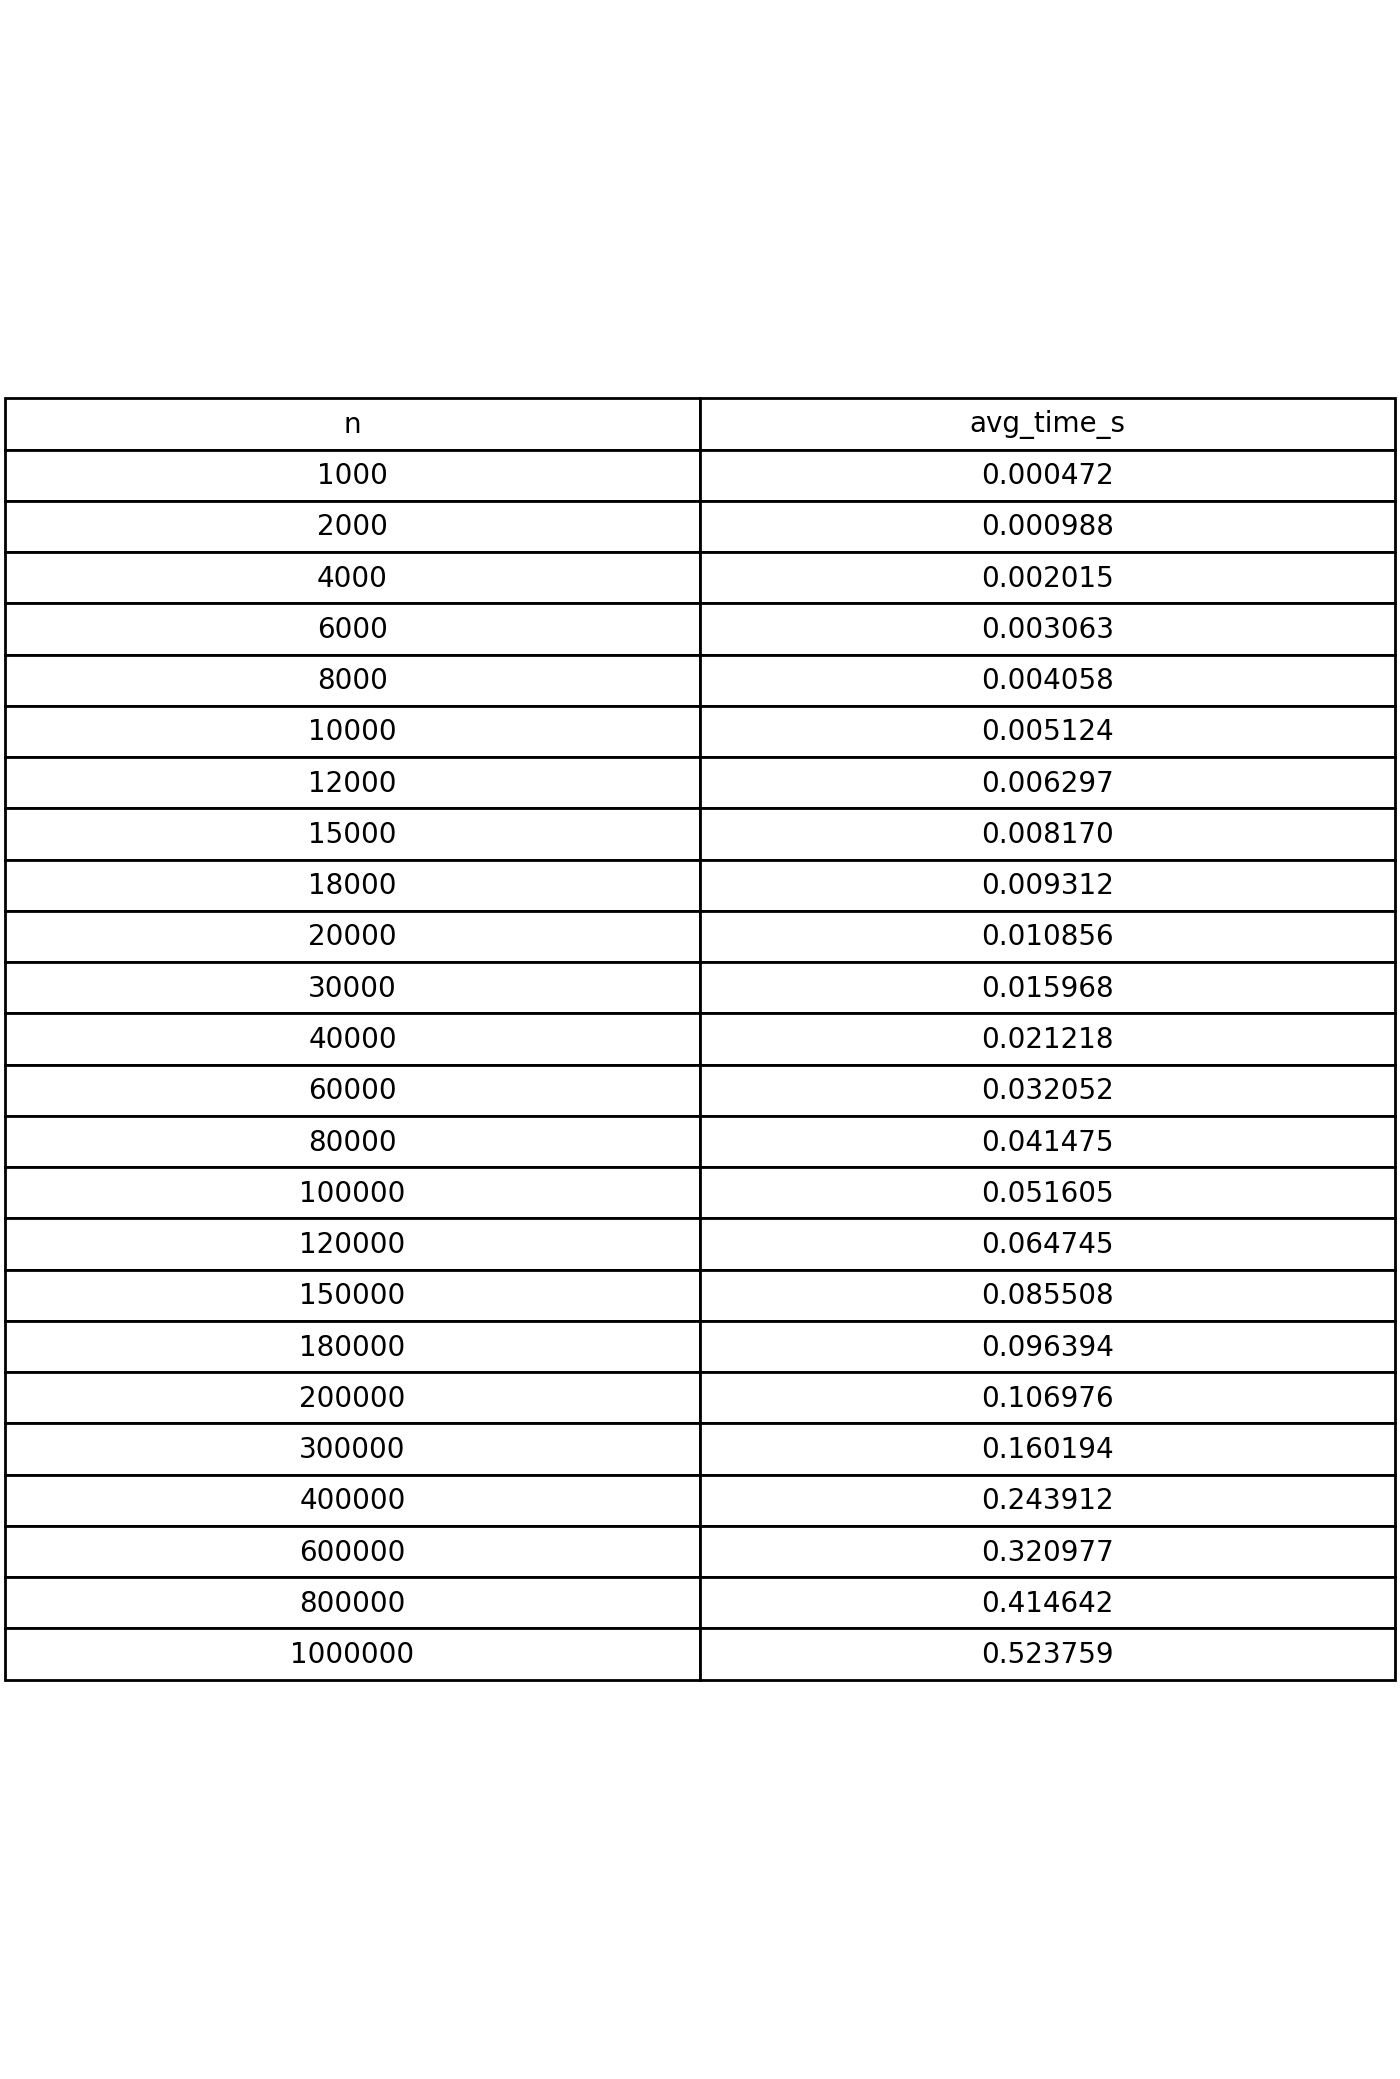
\includegraphics[width=0.8\textwidth]{bfs_table.png}
    \caption{Table of average execution times for BFS}
    \label{tab:bfs_results}
\end{figure}

\begin{figure}[H]
    \centering
    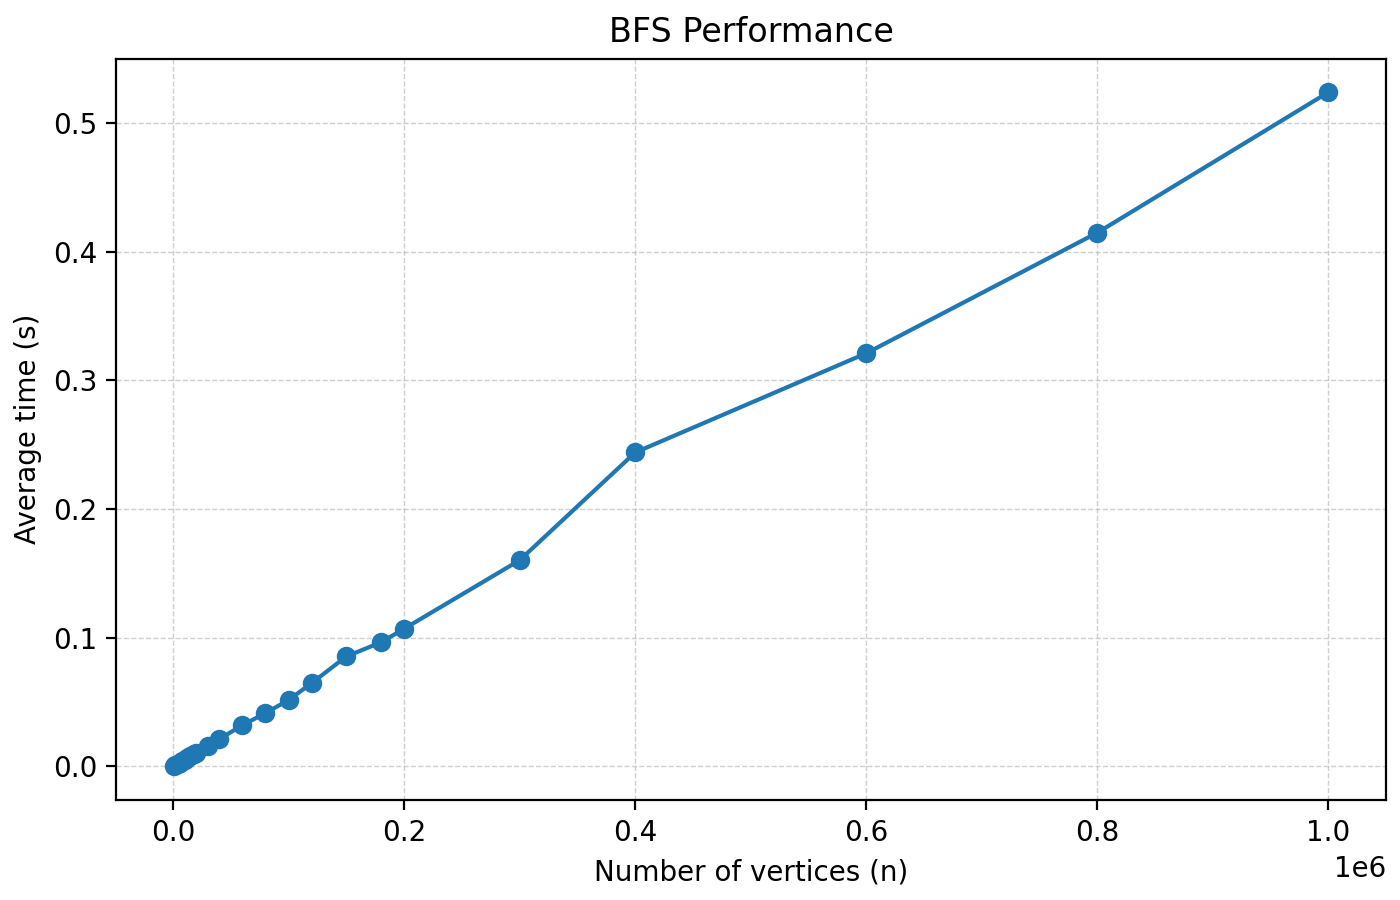
\includegraphics[width=0.8\textwidth]{bfs_graph.png}
    \caption{BFS performance graph}
    \label{fig:bfs_graph}
\end{figure}

The BFS graph shows approximately linear growth with the number of vertices, consistent with the theoretical complexity for sparse graphs.

\subsection{Depth First Search (DFS)}

\subsubsection{Algorithm Description}
The algorithm starts from a source node and explores neighbors deeply before backtracking. An explicit stack is used to avoid recursion depth issues.

Pseudocode:
\begin{verbatim}
DFS(graph, start):
    stack <- [start]
    while stack is not empty:
        u <- pop(stack)
        if visited[u]:
            continue
        visited[u] <- true
        for each v in graph[u]:
            if not visited[v]:
                push(stack, v)
\end{verbatim}

\subsubsection{Implementation}
\begin{lstlisting}[style=python, caption={DFS implementation in Python}]
DEGREE_STEPS = (3, 2, 1)

def dfs(node_count, start=0):
    node_count = int(node_count)
    if node_count <= 0:
        return 0

    start = int(start) % node_count
    visited = bytearray(node_count)
    stack = [start]
    visited_count = 0

    while stack:
        node = stack.pop()
        if visited[node]:
            continue

        visited[node] = 1
        visited_count += 1

        for step in DEGREE_STEPS:
            n_plus = (node + step) % node_count
            n_minus = (node - step) % node_count
            if not visited[n_plus]:
                stack.append(n_plus)
            if not visited[n_minus]:
                stack.append(n_minus)

    return visited_count
\end{lstlisting}

\subsubsection{Results}
\begin{figure}[H]
    \centering
    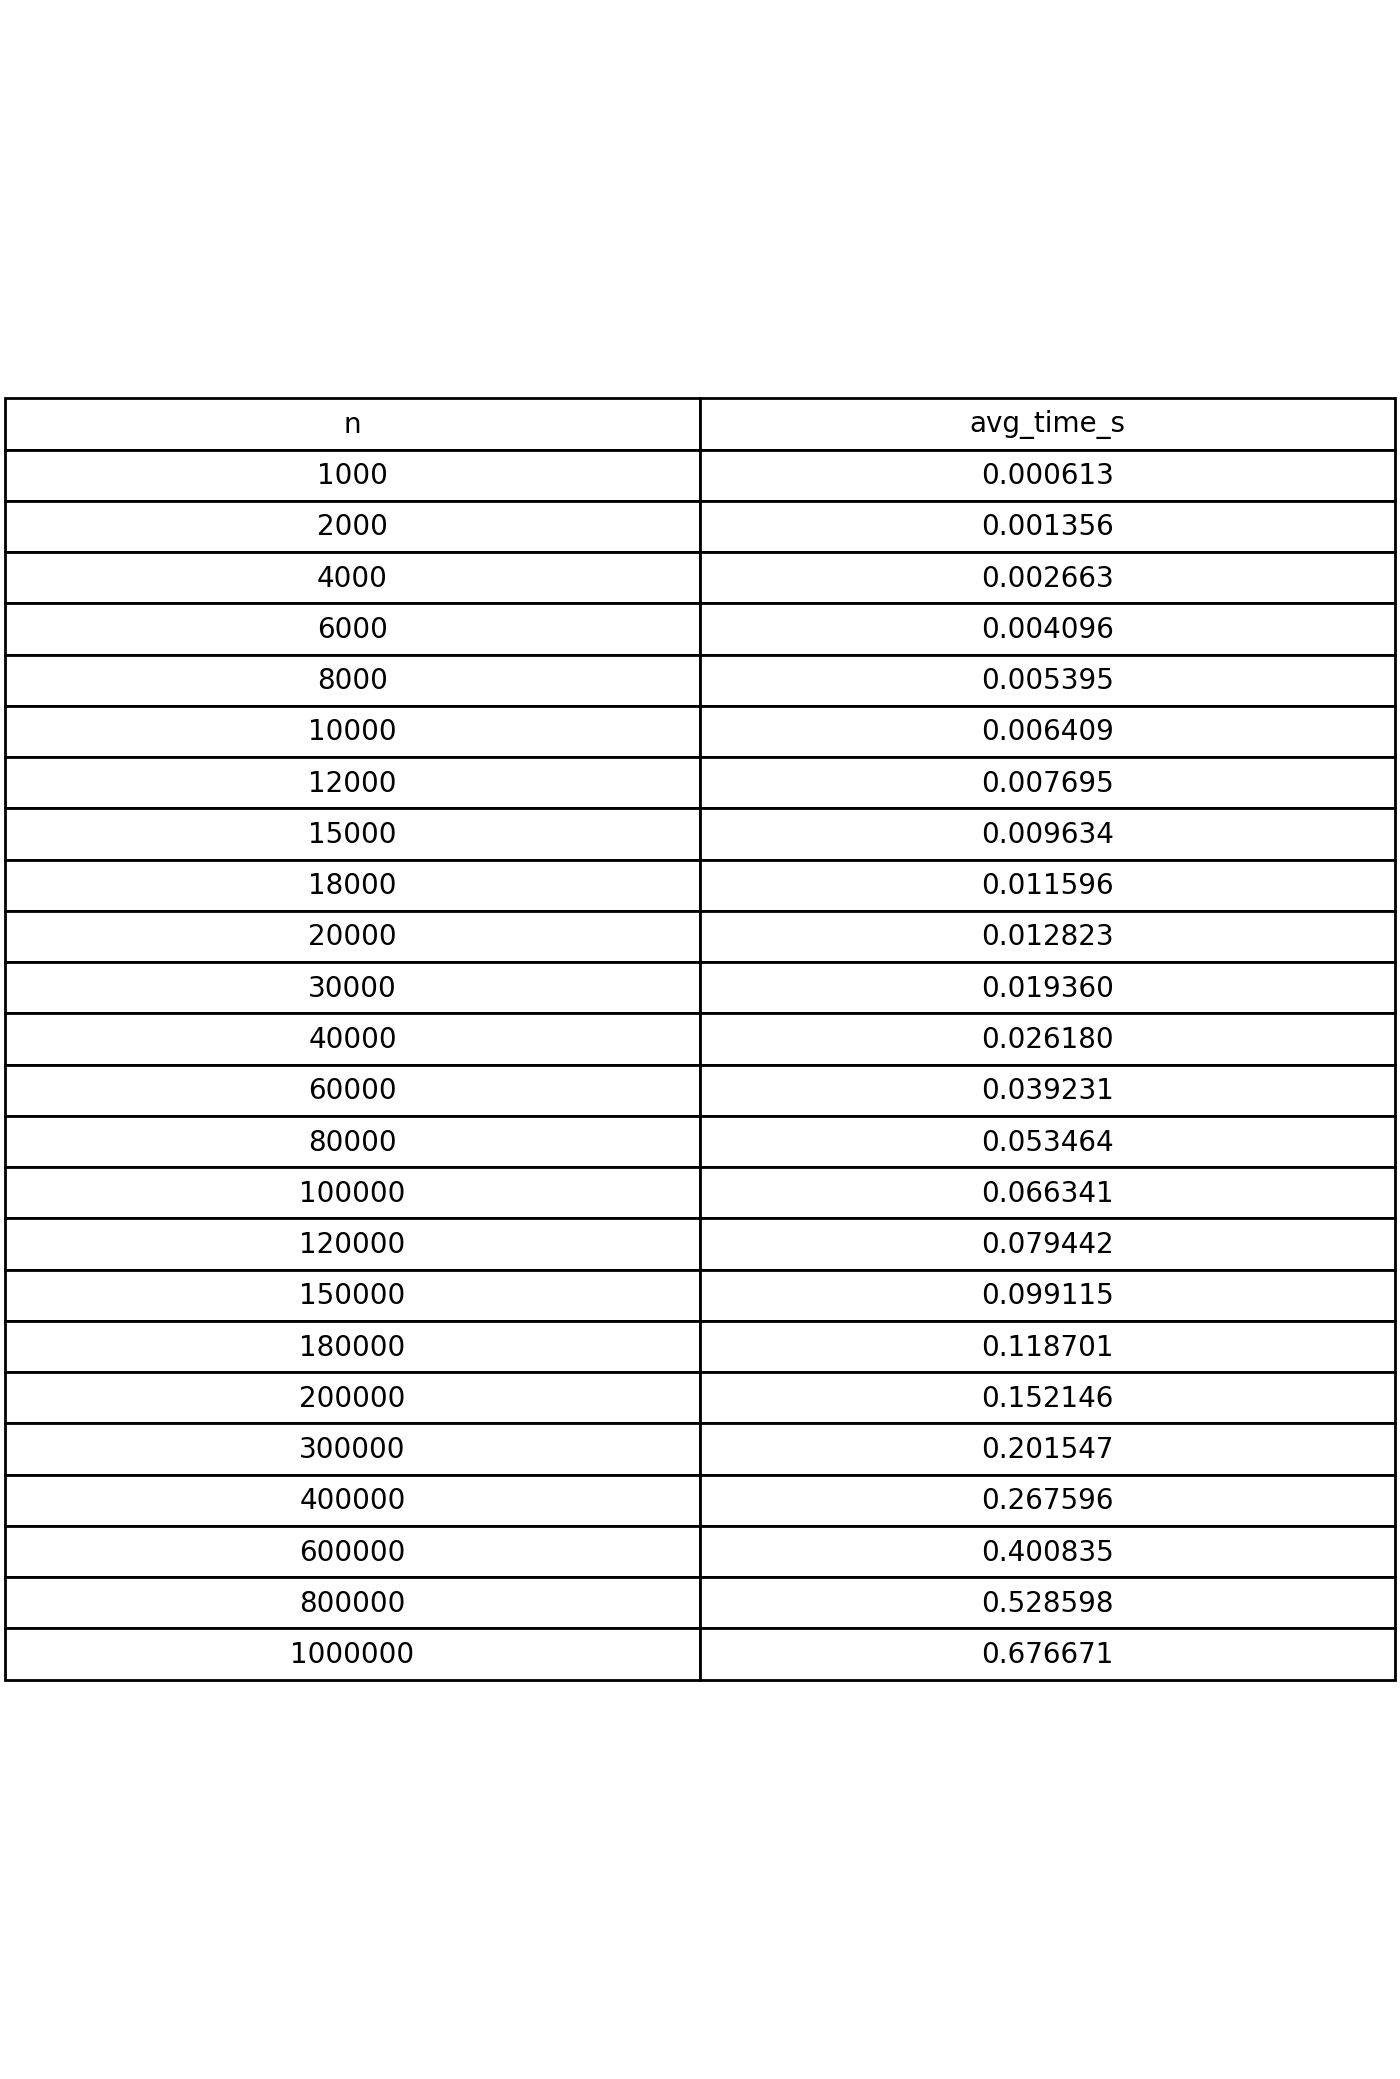
\includegraphics[width=0.8\textwidth]{dfs_table.png}
    \caption{Table of average execution times for DFS}
    \label{tab:dfs_results}
\end{figure}

\begin{figure}[H]
    \centering
    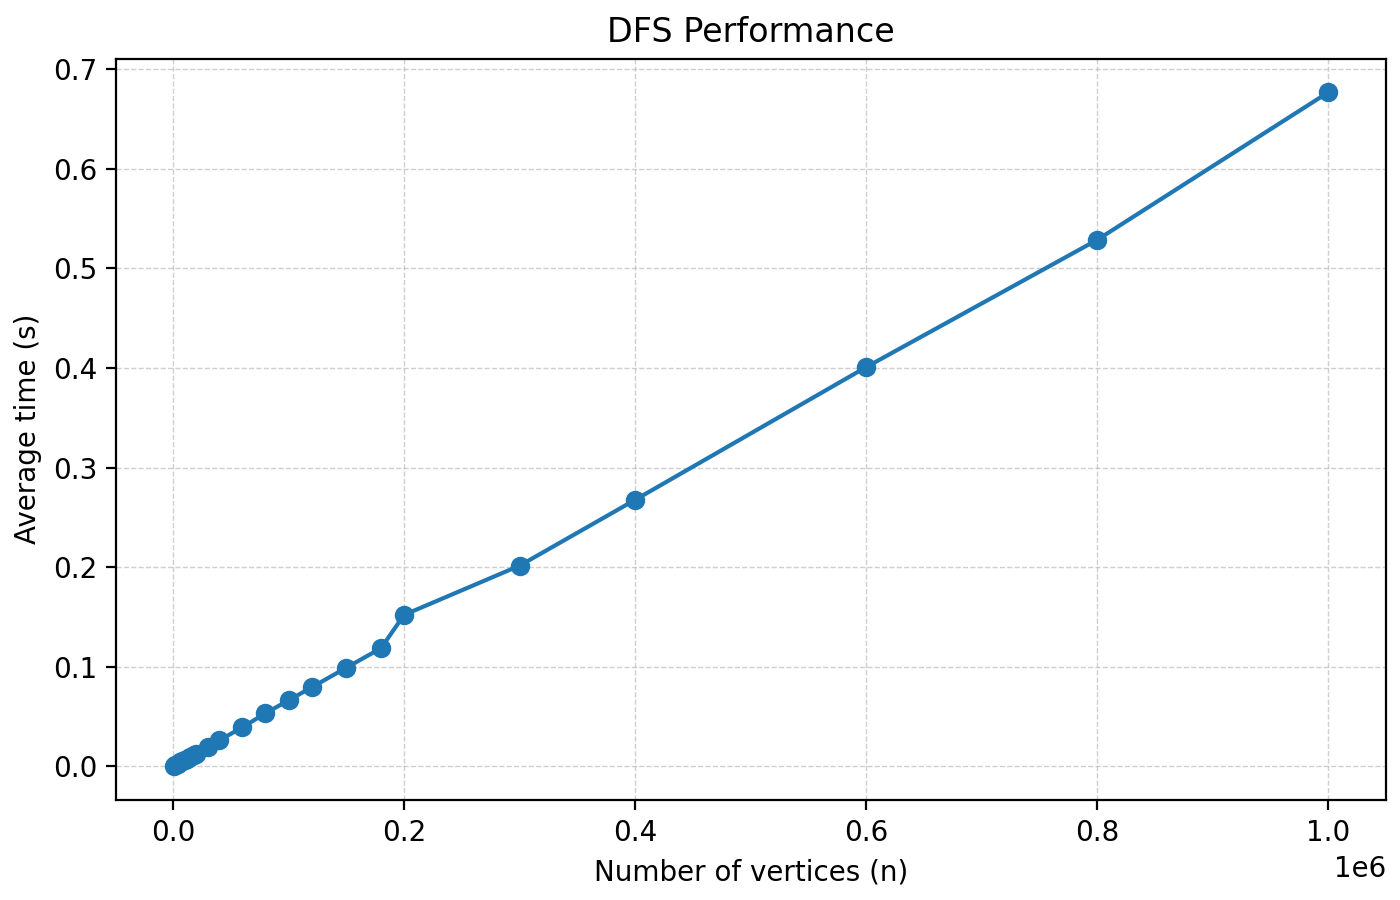
\includegraphics[width=0.8\textwidth]{dfs_graph.png}
    \caption{DFS performance graph}
    \label{fig:dfs_graph}
\end{figure}

The DFS graph also follows a near-linear trend, confirming expected behavior for sparse constant-degree graphs.

\subsection{Comparative Analysis}

\begin{figure}[H]
    \centering
    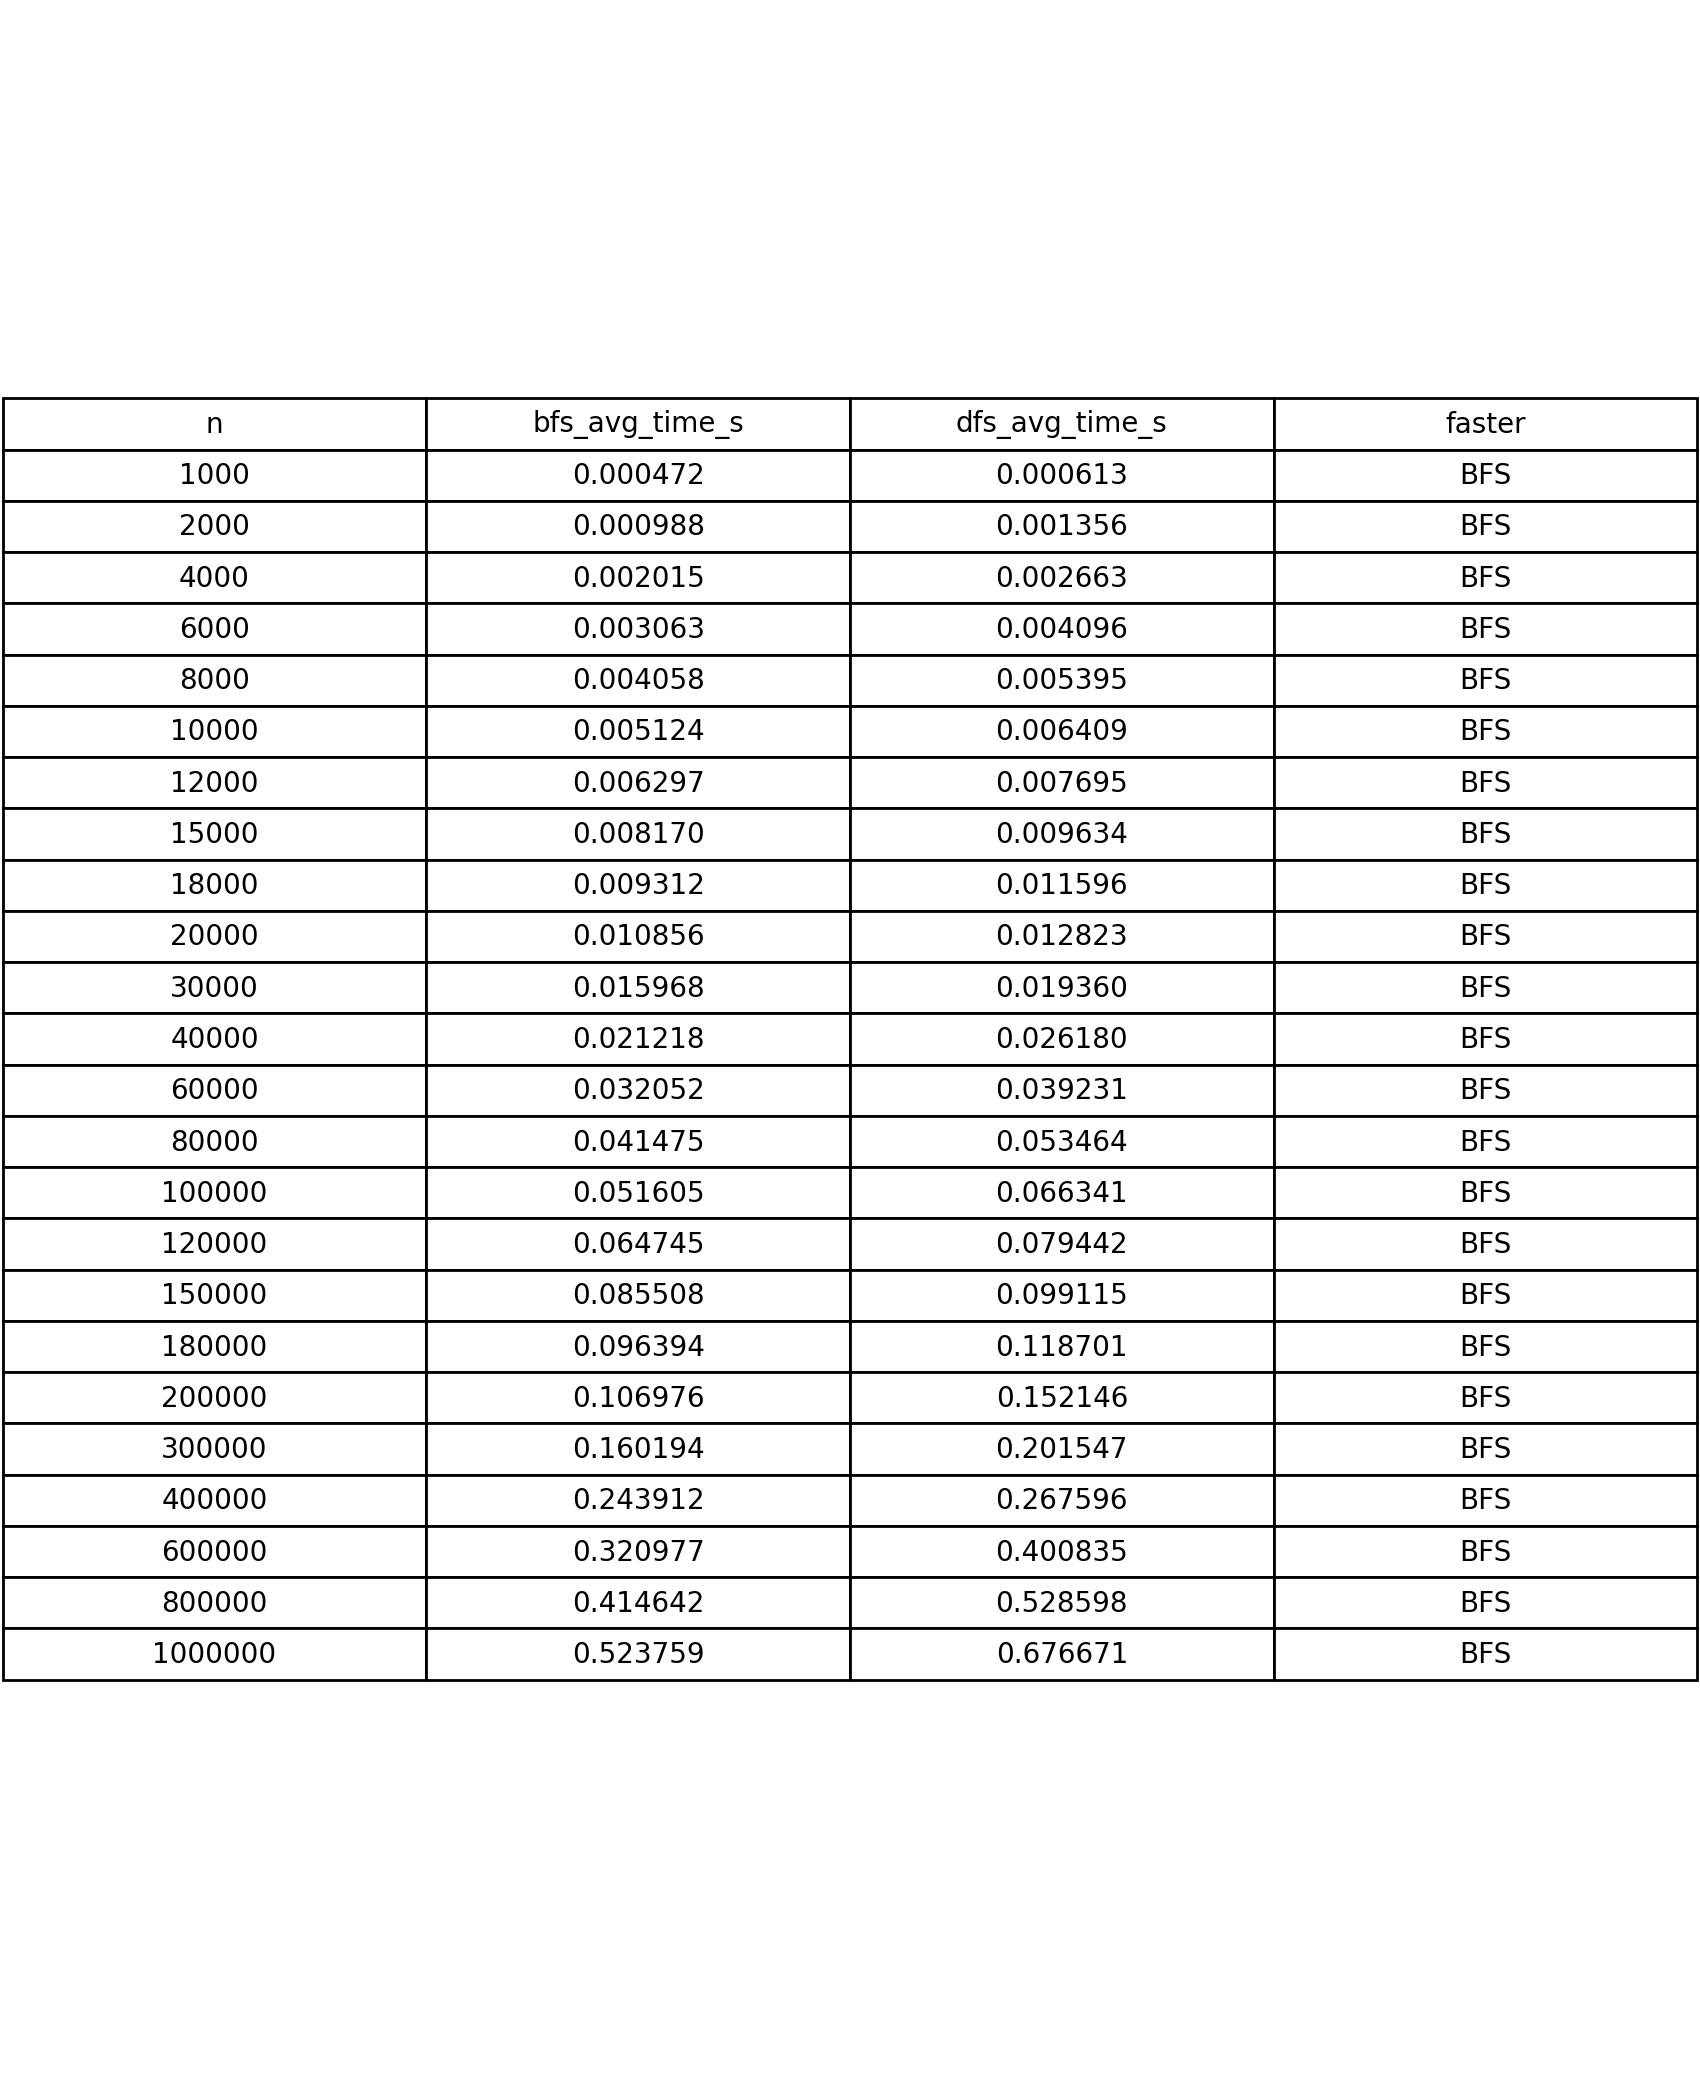
\includegraphics[width=0.95\textwidth]{comparison_table.png}
    \caption{BFS vs DFS measured times for each input size}
    \label{tab:comparison_results}
\end{figure}

\begin{figure}[H]
    \centering
    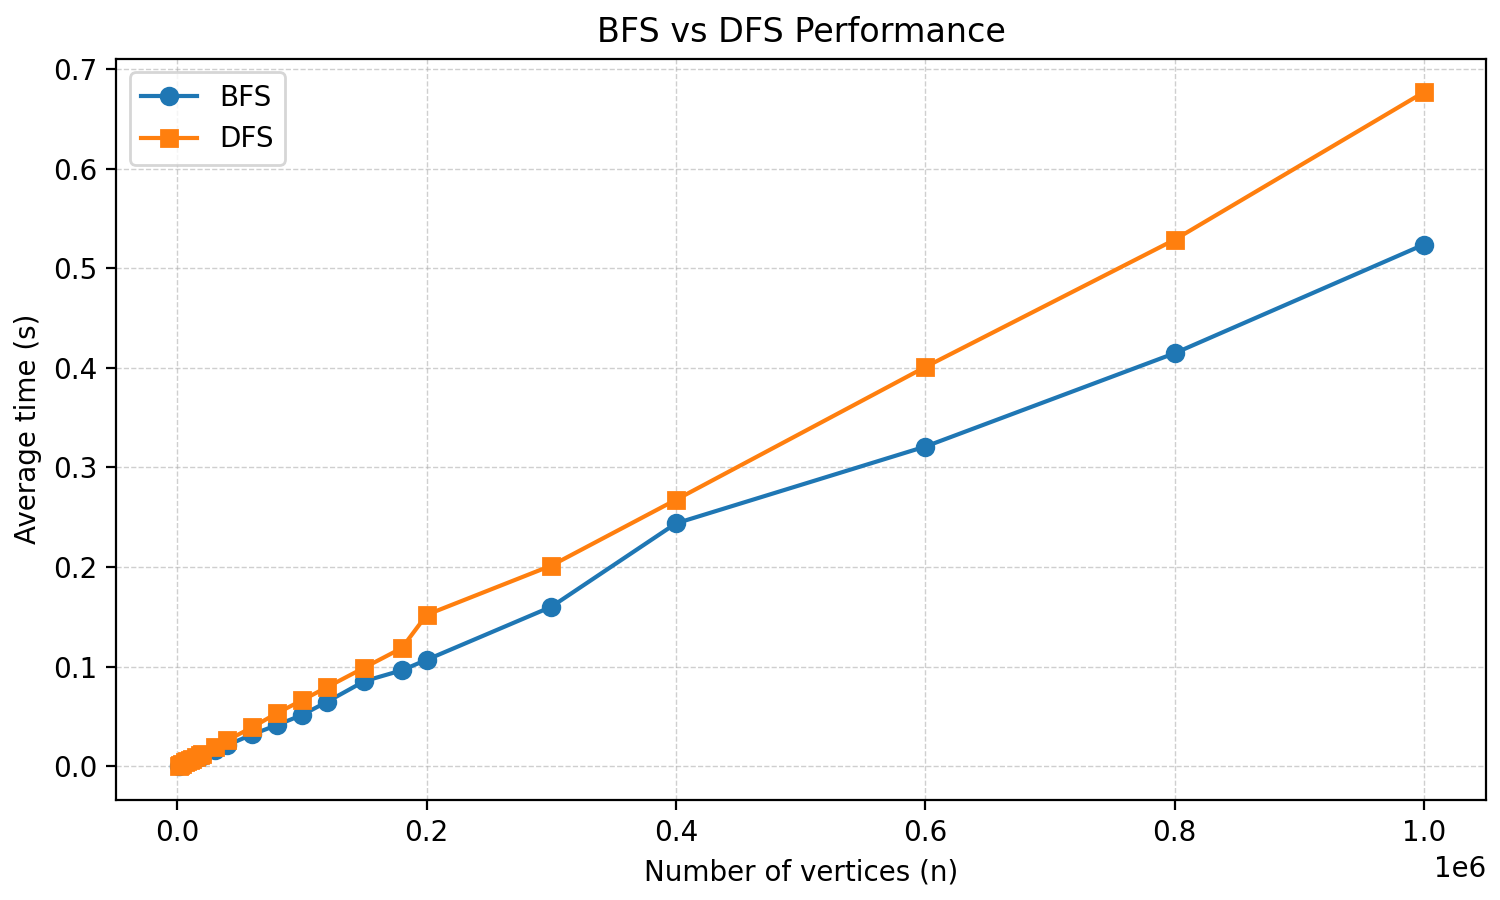
\includegraphics[width=0.8\textwidth]{comparison_graph.png}
    \caption{BFS and DFS performance comparison graph}
    \label{fig:comparison_graph}
\end{figure}

The comparison shows that BFS was consistently faster than DFS for all tested input sizes in this implementation. At the same time, both curves remain near-linear, which confirms the same asymptotic complexity class $O(V + E)$ and highlights differences in constant factors.

\subsection{Edge Case Analysis}

To validate robustness, several boundary and invalid-input scenarios were tested. The following implementation details explain most outcomes:
\begin{itemize}
    \item For non-positive sizes, both implementations return 0 immediately;
    \item For positive sizes, the start index is normalized with modulo $n$;
    \item Float parameters are supported through explicit normalization to integer indices.
\end{itemize}

\begin{figure}[H]
    \centering
    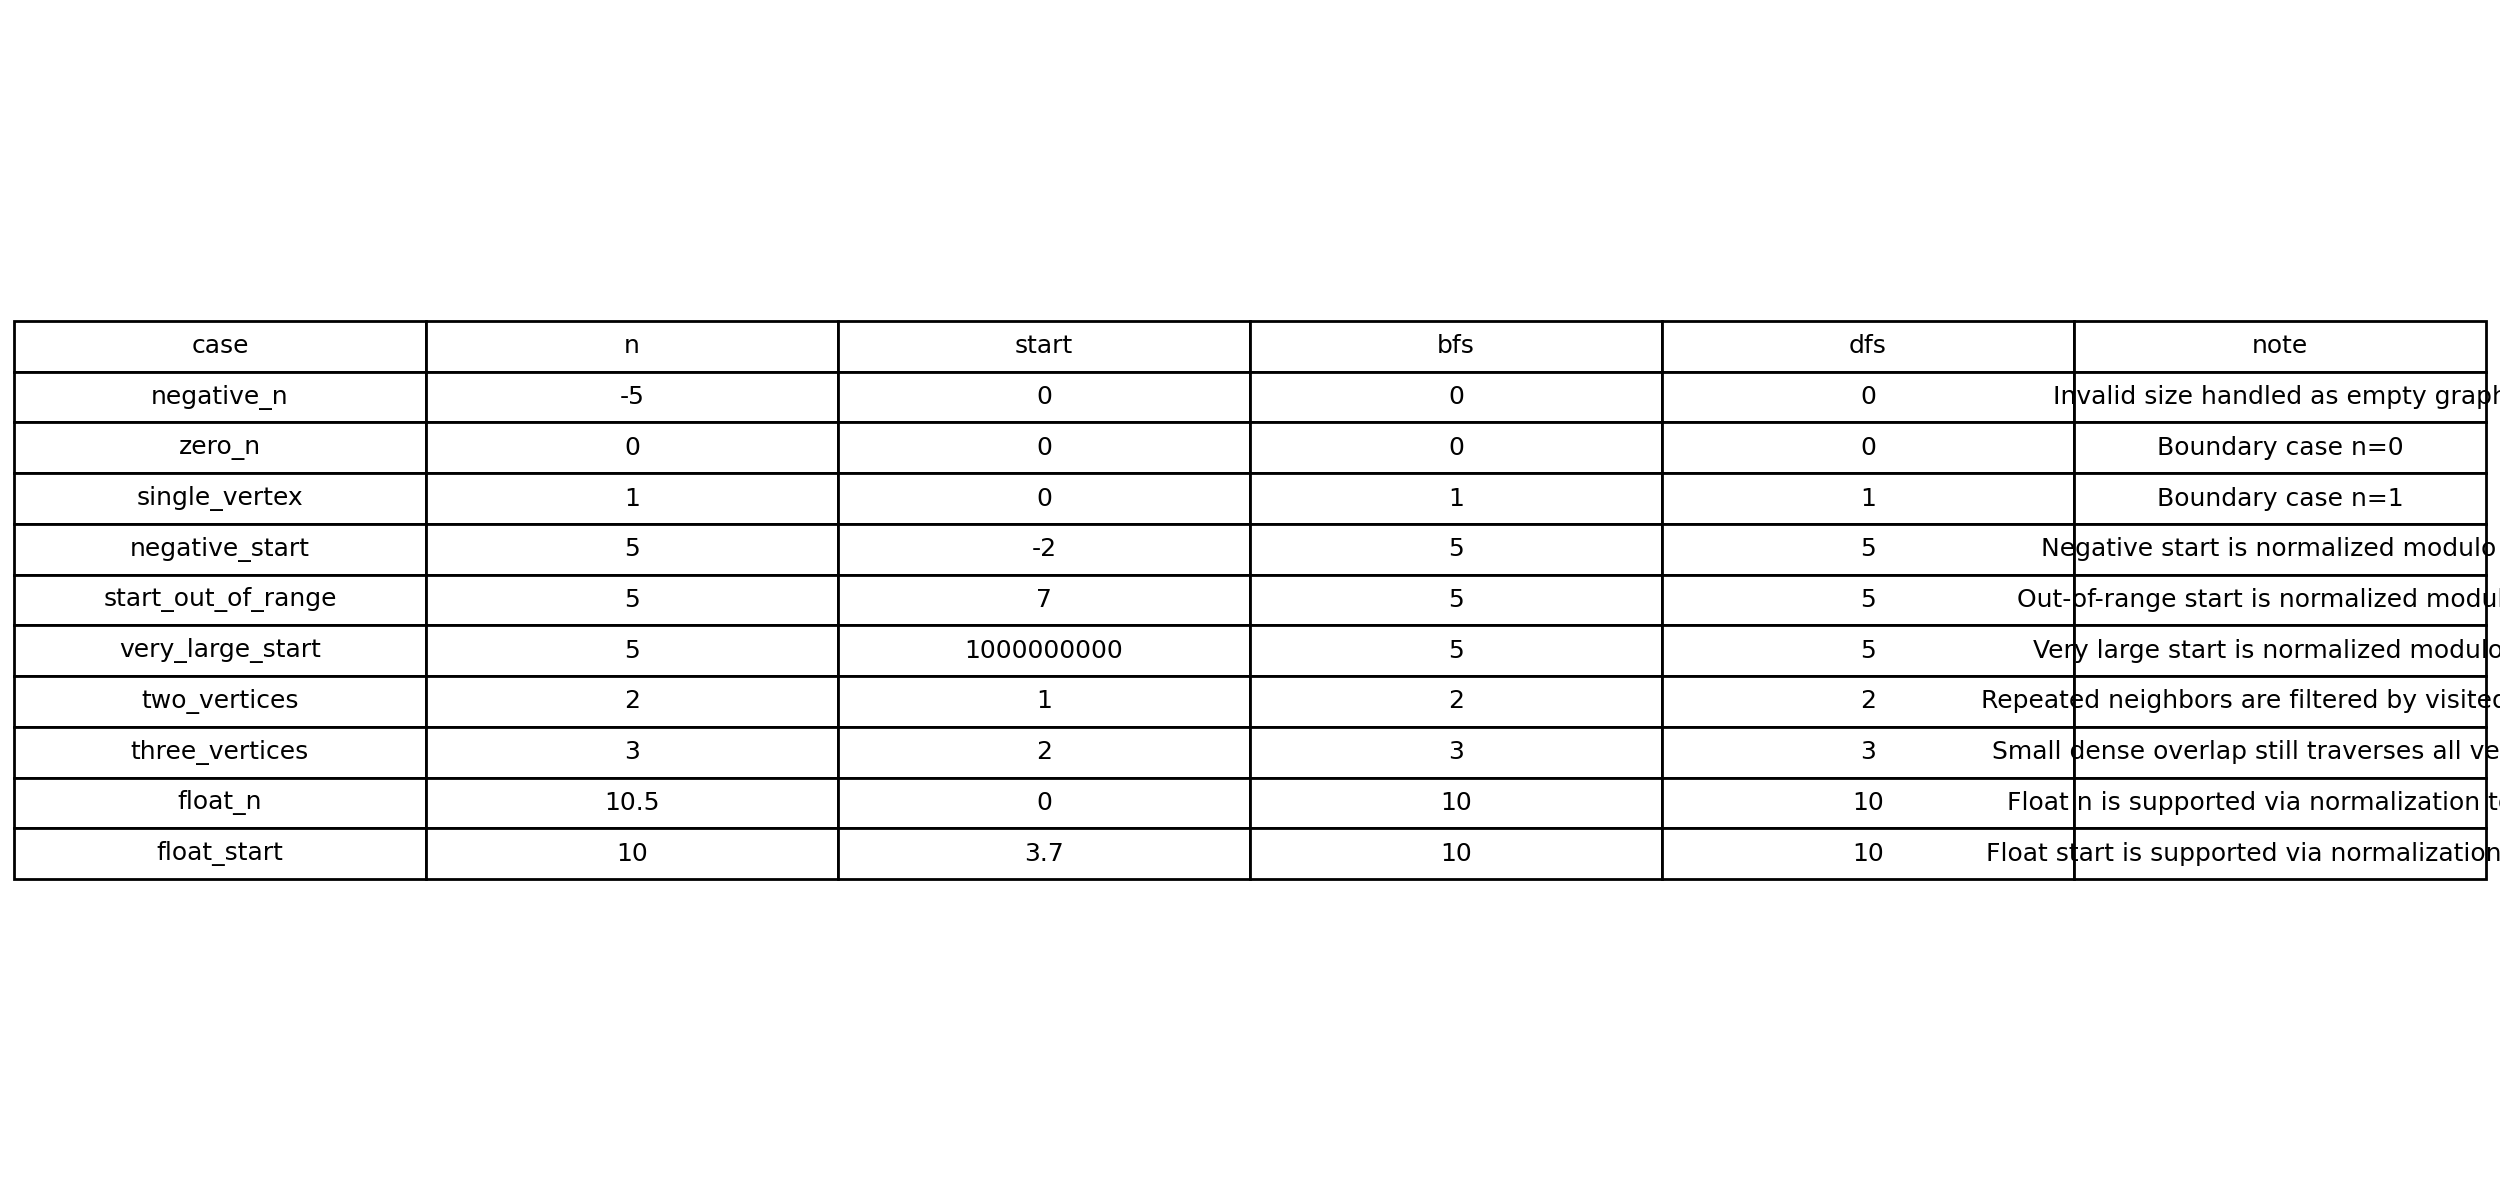
\includegraphics[width=\textwidth]{edge_cases_table.png}
    \caption{Edge-case behavior for BFS and DFS}
    \label{tab:edge_cases}
\end{figure}

The table confirms consistent behavior between BFS and DFS for boundary values ($n=0$, $n=1$), negative or oversized start indices, very small graphs where neighbors overlap heavily, and float parameters normalized to integer values.

\newpage
\section{CONCLUSION}

The laboratory objective was achieved by implementing BFS and DFS, defining input properties, selecting a comparison metric, running experiments, and presenting results graphically.

The measured data validates the theoretical complexity of both algorithms for sparse graphs: runtime grows approximately linearly with problem size when the degree remains constant.

From a practical perspective, BFS and DFS are both efficient for large sparse graphs, while BFS had a lower measured constant factor in this environment. The algorithm choice should still depend on task requirements: BFS for level-order exploration and shortest paths in unweighted graphs, DFS for deep exploration and structural graph analysis.

Edge-case testing also showed that both implementations are robust at boundaries and with normalized start indices, while still rejecting unsupported input types clearly.

\section*{Sources}
\begin{enumerate}
    \item \url{https://www.geeksforgeeks.org/breadth-first-search-or-bfs-for-a-graph/}
    \item \url{https://www.geeksforgeeks.org/depth-first-search-or-dfs-for-a-graph/}
    \item \url{https://www.youtube.com/watch?v=zaBhtODEL0w}
    \item \url{https://github.com/owhowh0/AALab3}
\end{enumerate}

\end{document}